% Intended LaTeX compiler: pdflatex
\documentclass[10pt,a4paper,UTF8]{article}
\usepackage{zclorg}
\author{张朝龙}
\date{}
\title{学习Python Doc第三天:函数}
\hypersetup{
 pdfauthor={张朝龙},
 pdftitle={学习Python Doc第三天:函数},
 pdfkeywords={},
 pdfsubject={},
 pdfcreator={Emacs 25.0.50.1 (Org mode 9.0.5)}, 
 pdflang={English}}
\begin{document}

\maketitle
\tableofcontents
\titlepic{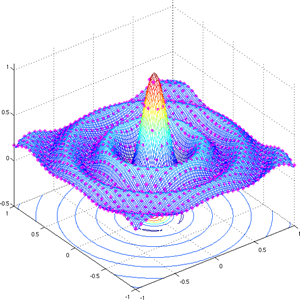
\includegraphics[scale=0.25]{../../img/sinc.PNG}}
\newpage

在定义函数的时候,我们可以为输入参数指定默认值,也可以使输入参数的个数可变,等等。今天,我们深入讨论一下函数。

\section{为函数指定默认参数值}
\label{sec:org65cf5f8}


在定义函数的时候可以为函数的一个或者多个参数指定默认值。通过这种方法,我们定义了一个可变参量的函数,在调用的时候,如果给定了默认值的参数没有被赋值则用默认值代替,看代码:
\lstset{language=Python,label= ,caption= ,captionpos=b,firstnumber=1,numbers=left}
\begin{lstlisting}
def ask_ok(prompt,retries=4,reminder='please try again'):
    while True:
        ok = input(prompt)
        if ok in ('y','ye','yes'):
            return True
        if ok in ('n','no','nop','nope'):
            return False
        retries = retries -1
        if retries < 0 :
            raise ValueError('invalid user response')
        print(reminder)
\end{lstlisting}

这个函数可以用三种方式调用:
\begin{enumerate}
\item 给定一个参数, \texttt{ask\_ok('Do you really want to quit?')}
\item 给一个可选参数赋值, \texttt{ask\_ok('OK to overwrite the file',2)}
\item 给所有参数赋值, \texttt{ask\_ok('OK to overwrite the file',2,'come on, only yes or no!')}
\end{enumerate}

这个函数在第 4 行引入了一个关键词 \texttt{in} ,这个关键词用来测试一个序列是不是包含了特定值。

参数的默认值在定义函数的时候就被执行了,看代码:
\lstset{language=Python,label= ,caption= ,captionpos=b,numbers=none}
\begin{lstlisting}
i = 5
def f(arg = i):
    print(arg)

i = 6
f()
\end{lstlisting}
输出为:
\begin{verbatim}
5
\end{verbatim}



可以看到 \texttt{arg=i} 中的 \texttt{i} 在定义的时候被赋值为 \texttt{5} 这个函数定义的时候就把 \texttt{arg} 赋值为 \texttt{5} 。

注意:默认值只被赋值一次。但是当默认参量是一个list,dictionary或者 大多数class的instance时 执行过程会稍有不同,看代码:
\lstset{language=Python,label= ,caption= ,captionpos=b,firstnumber=1,numbers=left}
\begin{lstlisting}
def f(a,L = []):
    L.append(a)
    return L

print(f(1))
print(f(2))
print(f(3))
\end{lstlisting}

输出为:
\begin{verbatim}
[1]
[1, 2]
[1, 2, 3]
\end{verbatim}
如果你不想在多次调用过程中共享默认值参量,你可以这样写:
\lstset{language=Python,label= ,caption= ,captionpos=b,firstnumber=1,numbers=left}
\begin{lstlisting}
def f(a,L = None ):
    if L is None:
        L = [];
    L.append(a)
    return L

print(f(1))
print(f(2))
print(f(3))
\end{lstlisting}
输出为:
\begin{verbatim}
[1]
[2]
[3]
\end{verbatim}
\section{关键词参数}
\label{sec:orgb97d96d}


关键词参数我还不是很理解,在python doc里有一个例子:
\lstset{language=Python,label= ,caption= ,captionpos=b,firstnumber=1,numbers=left}
\begin{lstlisting}
def parrot(voltage,state = 'a stiff', action = 'voom', type = 'Norwegian Blue'):
    print("-- This parrot wouldn't ", action, end=' ')
    print("if you put", voltage, "volts through it.")
    print("-- Lovely plumage, the", type)
    print("-- It's ",state,"!")
\end{lstlisting}

这个函数接受一个必选参数 \texttt{voltage} 和三个可选参数 \texttt{state} \texttt{action} \texttt{type} ,这个参数通过以下语句来调用:
\begin{verbatim}
parrot(1000)                                          # 1 positional argument
parrot(voltage=1000)                                  # 1 keyword argument
parrot(voltage=1000000, action='VOOOOOM')             # 2 keyword arguments
parrot(action='VOOOOOM', voltage=1000000)             # 2 keyword arguments
parrot('a million', 'bereft of life', 'jump')         # 3 positional arguments
parrot('a thousand', state='pushing up the daisies')  # 1 positional, 1 keyword
\end{verbatim}

但是下面的几种调用方式都是非法的:
\begin{verbatim}
parrot()                     # required argument missing
parrot(voltage=5.0, 'dead')  # non-keyword argument after a keyword argument
parrot(110, voltage=220)     # duplicate value for the same argument
parrot(actor='John Cleese')  # unknown keyword argument
\end{verbatim}

当一个函数的最后一个参数是 \texttt{**name} 这种类型时,该函数接受字典类型数据作为输入,看代码:
\lstset{language=Python,label= ,caption= ,captionpos=b,firstnumber=1,numbers=left}
\begin{lstlisting}
def cheeseshop(kind, *argument, **keywords):
    print("-- Do you have any",kind,"?")
    print("-- I'am sorry, we are all out of",kind)
    for arg in argument:
        print(arg)
    print('-'*40)
    keys = sorted(keywords.keys())
    for kw in keys:
        print(kw,":",keywords[kw])
\end{lstlisting}

调用时,可以这样子:
\begin{verbatim}
cheeseshop("Limburger", "It's very runny, sir.",
           "It's really very, VERY runny, sir.",
           shopkeeper="Michael Palin",
           client="John Cleese",
           sketch="Cheese Shop Sketch")
\end{verbatim}
输出为:
\begin{verbatim}
-- Do you have any Limburger ?
-- I'm sorry, we're all out of Limburger
It's very runny, sir.
It's really very, VERY runny, sir.
----------------------------------------
client : John Cleese
shopkeeper : Michael Palin
sketch : Cheese Shop Sketch
\end{verbatim}
\section{任意参数列表}
\label{sec:org487d3e0}


一个函数可以被设计的支持任意参数。这些参数被放置到一个tuple里。看代码:
\lstset{language=Python,label= ,caption= ,captionpos=b,firstnumber=1,numbers=left}
\begin{lstlisting}
def write_multiple_items(file, separator, *args):
    file.write(separator.join(args))
\end{lstlisting}

任何在 \texttt{*args} 之后出现的参数都被 \texttt{*args} 接受。另外在定义函数时, \texttt{*args} 之后的参数必须以 \texttt{keyword-value} 的形式出现。

比如:
\lstset{language=Python,label= ,caption= ,captionpos=b,firstnumber=1,numbers=left}
\begin{lstlisting}
def concat(*args,sep = "/"):
    return sep.join(args)
\end{lstlisting}
调用和输出为:
\begin{verbatim}
In [333]: concat("earth","mars","venus")
Out[337]: 
'earth/mars/venus'

In [338]: concat("earth","mars","venus",sep='.')
Out[356]: 
'earth.mars.venus'
\end{verbatim}
\section{Lambda 表达式}
\label{sec:orgb84aaf1}


可以使用 \texttt{lambda} 来表示一些小的匿名函数。比如 \texttt{lambda a,b: a+b} 返回 \texttt{a,b} 的和。 \texttt{lambda} 可以被用在对象调用的地方。从语法上来看, \texttt{lambda} 表达式是一句话。 \texttt{python} 中的 \texttt{lambda} 有点语法糖的味道。一个简单的例子,看代码:
\lstset{language=Python,label= ,caption= ,captionpos=b,firstnumber=1,numbers=left}
\begin{lstlisting}
def make_incrementor(n):
    return lambda x: x+n
\end{lstlisting}

调用和输出为:
\begin{verbatim}
In [1]: 
In [2]: f = make_incrementor(42)

In [33]: f(0)
Out[33]: 
42

In [34]: f(1)
Out[34]: 
43

In [35]: f(4)
Out[38]: 
46
\end{verbatim}

\texttt{make\_incrementor} 生成的是一个 \texttt{generator} .

\section{代码文档格式规范化}
\label{sec:org3565b61}


在写 \texttt{Python} 代码的过程中,可以顺便把代码文档也给完成,颇有文学编程的感觉。对于函数来说可以通过以下方式告知该函数的信息:
\lstset{language=Python,label= ,caption= ,captionpos=b,firstnumber=1,numbers=left}
\begin{lstlisting}
def my_function():
    """ Do nothing, it doesn't do anything

    no, really, it doesn't do anything
    """

    pass
\end{lstlisting}

通过 \texttt{print(my\_function.\_\_doc\_\_)} 查看 \texttt{my\_function} 的文档:
\begin{verbatim}
In [40]: print(my_function.__doc__)
 Do nothing, it doesn't do anything

    no, really, it doesn't do anything
\end{verbatim}


当 \texttt{Python} 工程较大时,更需要规范化的文档和编程风格。所幸 \texttt{PEP 8} 提供了高度可读的编码风格,每个 \texttt{python} 程序员都应当遵守这个规范(尤其参与大项目的时候,像我平常做的小实验,我就不那么严格的要求了)。
\end{document}
